%*****************************************
\chapter{Data Cleaning}\label{ch:datacleaning}
%*****************************************

\section{Intro}

In the previous section we have described which type of data is available to us. In here we are going to explain how the data is clean and transformed into something more useful.\vspace{3 mm}

The process consist into importing the data from the files described previously with no type of filter. Then transforming the original data into values that are more meaningful, as well as adding new columns to our data based on data that we already have. For example, whether a person is SA carrier or not. Then preprocessing the data and adding columns that are time intensive. For example, searching for all the friends of a person and counting how many follow him, takes a lot of computational time when you have to do it thousands of times, but you don't need to do this every time you run the network analysis. You can precalculate it only once, add the number to your data, and have it ready forever.\vspace{3 mm}

After this, the data is finally clean and ready, but we don't use the data yet. We save this final version into CSV files and later the analysis will read these files every time is called. This way, the data cleaning, the filtering, and analysis are independent from each other. Later on, during the analysis you can further filter or stratify the data to whatever you want.\vspace{3 mm}

\begin{figure}[H]
{
    \centering

    \label{fig:Data_cleaning_summary}

    \includegraphics[width=1\textwidth]{../img/figures/cleaning.png}
    \caption{Summarize of the data cleaning process}
}
\medskip
\end{figure}

In all cases, first we are going to change the selected variable names to something more meaningful; the same for the categorical values that are encoded as numbers.\vspace{3 mm}

In the particular case of the School variable, the original titles described in the metadata as "Specialization in General Studies", "Vocational Program", and "Sports and Physical Education" are too long, and the plots become difficult to read. So they will be simplified to shorter texts. \vspace{3 mm}

\section{Naming}

First we are going to review all the names changes. To keep consistency, we are going to keep the same order and tables use in the Metadata chapter. \vspace{3 mm}


\subsection{Basic information}

\begin{table}[H]
    \centering

    \label{table:Basic_info_new_names}
    
	\renewcommand{\arraystretch}{1.5}

    \begin{tabular}{| l | l }
        \hline
        \rowcolor[HTML]{FFAAAA}

        \textbf{Original Name} & \textbf{New Name} \\ 
        \hline 

        \multicolumn{1}{l|}{\detokenize{pers_key_ff1}} & ID      \\ 
        \multicolumn{1}{l|}{\detokenize{SEX_FF1}}      & Sex     \\ 
        \multicolumn{1}{l|}{\detokenize{AGE_FF1}}      & Age     \\ 


    \end{tabular}%

    \caption{Table with the new names the basic information variables.}
    
\end{table}

\subsection{School and education}

\begin{table}[H]
    \centering

    \label{table:school_and_education_new_names}

	\renewcommand{\arraystretch}{1.5}

    \begin{tabular}{| l | p{0.5\linewidth}  l }
    
    
    
        \hline
        \rowcolor[HTML]{FFAAAA}

        \textbf{Original Name} & \textbf{New Name} \\ 
        \hline 

        \multicolumn{1}{l|}{\detokenize{HIGH_SCHOOL_NAME_FF1}}         & HighSchoolID \\ 
        \multicolumn{1}{l|}{\detokenize{HIGH_SCHOOL_CLASS_FF1}}        & Class        \\ 
        \multicolumn{1}{l|}{\detokenize{HIGH_SCHOOL_PROGRAMME_FF1}}    & Not used. This is actually not defined in the metadata and we can't find what each number means. \\ 
        \multicolumn{1}{l|}{\detokenize{HIGH_SCHOOL_MAIN_PROGRAM_FF1}} & School       \\ 

    \end{tabular}%
    

    \caption{Table with the new names for the education variables.}
    
\end{table}

\subsection{Recreational Drugs}

\begin{table}[H]
    \centering

    \label{table:Recreational_drugs_new_names}
    
	\renewcommand{\arraystretch}{1.5}

    \begin{tabular}{| l | l }
        \hline
        \rowcolor[HTML]{FFAAAA}

        \textbf{Original Name} & \textbf{New Name} \\
        \hline 

        \multicolumn{1}{l|}{\detokenize{SMOKE_FF1}}             & Smoke   \\ 
        \multicolumn{1}{l|}{\detokenize{SNUFF_FF1}}             & Snuff   \\ 
        \multicolumn{1}{l|}{\detokenize{ALCOHOL_FREQUENCY_FF1}} & Alcohol \\ 

    \end{tabular}%

    \caption{Table with the new names for the recreational drugs variables.}
    
\end{table}

\subsection{Physical Activity}

\begin{table}[H]
    \centering

    \label{table:Physical_activity_info_new_names}
    
	\renewcommand{\arraystretch}{1.5}

    \begin{tabular}{| l | p{10cm}  l }
        \hline
        \rowcolor[HTML]{FFAAAA}

        \textbf{Original Name} & \textbf{New Name} \\
        \hline 

        \multicolumn{1}{l|}{\detokenize{PHYS_ACT_LEISURE_FF1}}         & Sports \\ 
		\multicolumn{1}{l|}{\detokenize{PHYS_ACT_OUTSIDE_SCHOOL_FF1}}  & Active \\ 

    \end{tabular}%

    \caption{Table with the new names for the physical information variables.}
    
\end{table}

\subsection{Anthropometry}

\begin{table}[H]
    \centering

    \label{table:Anthropometry_new_names}
    
	\renewcommand{\arraystretch}{1.5}

    \begin{tabular}{| l | l }
        \hline
        \rowcolor[HTML]{FFAAAA}

        \textbf{Original Name} & \textbf{New Name} \\
        \hline 

        \multicolumn{1}{l|}{\detokenize{HEIGHT_FF1}} & Height       \\
        \multicolumn{1}{l|}{\detokenize{WEIGHT_FF1}} & Weight       \\         
        \multicolumn{1}{l|}{\detokenize{WAIST1_FF1}} & Waist. Averaged with WAIST2  \\         
        \multicolumn{1}{l|}{\detokenize{HIP1_FF1}}   & Hip. Averaged with HIP2      \\         
        \multicolumn{1}{l|}{\detokenize{WAIST2_FF1}} & Not used.    \\         
        \multicolumn{1}{l|}{\detokenize{HIP2_FF1}}   & Not used.    \\         
        \multicolumn{1}{l|}{\detokenize{BMI_FF1}}    & BMI          \\ 
        
            
    \end{tabular}%

    \caption{Table with the new names anthropometric variables.}

\end{table}


\subsection{Medicines}

Medicines goes into an special table because in the current data format doesn't meet the basic normalization standards for databases. Nevertheless, some of the variables can be kept in the main table.\vspace{3 mm}

\begin{table}[H]
    \centering

    \label{table:Medicines_new_names}
    
	\renewcommand{\arraystretch}{1.5}

    \begin{tabular}{| l | p{10cm}  l }
        \hline
        \rowcolor[HTML]{FFAAAA}

        \textbf{Original Name} & \textbf{New Name} \\
        \hline 

		\multicolumn{1}{l|}{\detokenize{ANTIBIOTICS_FF1}}         & Antibiotics \\ 
		\multicolumn{1}{l|}{\detokenize{ANTIBIOTICS_BRAND1_FF1}}  & AntiBrand \\ 	
		\multicolumn{1}{l|}{\detokenize{ANTIBIOTICS_ATC1_FF1}}    & AntiATC \\		
		\multicolumn{1}{l|}{\detokenize{ANTIBIOTICS_BRAND2_FF1}}  & Not in use. Nobody takes a second antibiotic. \\
		\multicolumn{1}{l|}{\detokenize{ANTIBIOTICS_ATC2_FF1}}    & Not in use \\ 
		\multicolumn{1}{l|}{\detokenize{MEDICATION_DAILY_FF1}}    & TotalMedication (see later) \\
		\multicolumn{1}{l|}{\detokenize{MEDICATION_BRAND1_FF1}}   & (See later) \\ 
		\multicolumn{1}{l|}{\detokenize{MEDICATION_ATC1_FF1}}	  & (See later) \\ 
		\multicolumn{1}{l|}{\detokenize{MEDICATION_REGULAR1_FF1}} & (See later) \\ 

        \multicolumn{1}{l|}{\detokenize{ -- Rest of regular medicines --}}
        & The previous rows repeat for Regular medicines 1, 2, 3, 4, and 5.\\		

		\multicolumn{1}{l|}{\detokenize{MEDICATION_OTHER_FF1}}   & Not in use. See next \\ 
		
		\multicolumn{1}{l|}{\detokenize{MEDICATION_OTHER_DESC_FF1}}
		& Not in use. Most of the people tell redundant medication already registered in the other medicine variables, or in the contraceptives variables. Others take seasonal drugs for allergies. Nobody answer this column with actual information about bizarre combinations of drugs.\\

    \end{tabular}%

    \caption{Table with the new names for medicine intake related variables.}

\end{table}

To ensure Boyce-Codd normal form of the medical data, we create this new table where we store the medical data of everyone. As such, the previous variable TotalMedication doesn't tell you just if a person takes medicine or not only, it tells you how many different drugs.\vspace{3 mm}

\begin{table}[H]
    \centering

    \label{table:Medicines_new_relational_table}
    
	\renewcommand{\arraystretch}{1.5}

    \begin{tabular}{| l | p{10cm}  l }
        \hline
        \rowcolor[HTML]{FFAAAA}

        \textbf{Original Name} & \textbf{New Name} \\
        \hline 

        \multicolumn{1}{l|}{\detokenize{pers_key_ff1}} & ID      \\ 
		\multicolumn{1}{l|}{\detokenize{MEDICATION_BRAND1_FF1}}   & Brand \\ 
		\multicolumn{1}{l|}{\detokenize{MEDICATION_ATC1_FF1}}	  & ATC \\ 
		\multicolumn{1}{l|}{\detokenize{MEDICATION_REGULAR1_FF1}} & Regularity \\ 
		\multicolumn{1}{l|}{\detokenize{MEDICATION_REGULAR1_FF1}} & Content \\ 

    \end{tabular}%

    \caption{Table with the new names for the new drugs intake related variables table.}

\end{table}


\subsection{Diseases}

Diseases also have the same lack of normalization of the data as medicine. As such, we transform this the same way. There is a significant difference though, the OTHER variables are actually very relevant here, and we need to clean them up manually. Furthermore, the \detokenize{CHRONIC_DISEASE_FF1} is worthless and doesn't have consistency with the data.\vspace{3 mm}

\begin{table}[H]
    \centering

    \label{table:Diseases_new_names}
    
	\renewcommand{\arraystretch}{1.5}

    \begin{tabular}{| l | p{10cm}  l }
        \hline
        \rowcolor[HTML]{FFAAAA}

        \textbf{Original Name} & \textbf{New Name} \\
        \hline 


		\multicolumn{1}{l|}{\detokenize{CHRONIC_DISEASE_FF1}}            & TotalDiseases \\ 		
		\multicolumn{1}{l|}{\detokenize{DIAGNOSIS_CHRONIC_DISEASE1_FF1}} & (See later)   \\ 
		\multicolumn{1}{l|}{\detokenize{ICD10_CHRONIC_DISEASE1_FF1}}     & (See later)   \\
		
        \multicolumn{1}{l|}{\detokenize{ -- Rest of Chronic Diseases --}}
        & The previous rows repeat for Chronic Disease 1, 2, 3, 4, and 5.\\		

		\multicolumn{1}{l|}{\detokenize{CHRONIC_DISEASE_OTHER_FF1}}		 & Not used       \\ 
		
		\multicolumn{1}{l|}{\detokenize{CHRONIC_DISEASE_OTHER_DESC_FF1}} & (See later) \\

		\multicolumn{1}{l|}{\detokenize{DIABETES_FF1}}
		& Not used. Already in the diseases table, which include type (all are type 1). \\

		\multicolumn{1}{l|}{\detokenize{ICHY_SKIN_FF1}}
		& Not used. Already in the diseases table covered by several diseases. \\ 
		
		\multicolumn{1}{l|}{\detokenize{ICHY_SKIN_LOCATION_FF1}}
		& Not used. \\ 
		
		\multicolumn{1}{l|}{\detokenize{PSORIASIS_LIFETIME_FF1}}
		& Not used. Already in the diseases table. \\
		
        \multicolumn{1}{l|}{\detokenize{PSORIASIS_SEVERITY_FF1}}
        & Not used.\\		

		\multicolumn{1}{l|}{\detokenize{ALLERGIC_RHINITIS_FF1}}
		& Not used. Already in the diseases table. \\
		
		\multicolumn{1}{l|}{\detokenize{ASTHMA_FF1}}
		& Not used. Already in the diseases table. \\

		\multicolumn{1}{l|}{\detokenize{ATOPIC_ECZEMA_FF1}}
		& Not used. Already in the diseases table. \\
            
            
    \end{tabular}%

    \caption{Table with the new names for diseases related variables.}

\end{table}

As with the medicine table, we created a proper normalization table for diseases.\vspace{3 mm}

\begin{table}[H]
    \centering

    \label{table:Diseases_new_relational_table}
    
	\renewcommand{\arraystretch}{1.5}

    \begin{tabular}{| l | p{10cm}  l }
        \hline
        \rowcolor[HTML]{FFAAAA}

        \textbf{Original Name} & \textbf{New Name} \\
        \hline 

        \multicolumn{1}{l|}{\detokenize{pers_key_ff1}}                   & ID         \\ 
		\multicolumn{1}{l|}{\detokenize{DIAGNOSIS_CHRONIC_DISEASE1_FF1}} & Diagnostic \\ 
		\multicolumn{1}{l|}{\detokenize{ICD10_CHRONIC_DISEASE1_FF1}}	 & ICD10      \\ 
		\multicolumn{1}{l|}{\detokenize{ICD10_CHRONIC_DISEASE1_FF1}}	 & Title      \\ 


    \end{tabular}%

    \caption{Table with the new names for the new drugs intake related variables table.}

\end{table}



\subsection{Menstrual cycle}

\begin{table}[H]
    \centering

    \label{table:Menstrual_info_new_names}
    
	\renewcommand{\arraystretch}{1.5}

    \begin{tabular}{| l | p{10cm}  l }
        \hline
        \rowcolor[HTML]{FFAAAA}

        \textbf{Original Name} & \textbf{New Name} \\
        \hline 

        \multicolumn{1}{l|}{\detokenize{MENSES_FF1}} & Menstruating \\ 
        \multicolumn{1}{l|}{\detokenize{MENSES_REGULARITY_FF1}} & MenstruationRegular \\ 
        \multicolumn{1}{l|}{\detokenize{MENSES_CYCLE_LENGTH_FF1}} & MenstruationCycle \\ 
        \multicolumn{1}{l|}{\detokenize{MENSES_START_DATE_CERTAIN_FF1}}
        & Not used, redundant information (see next) \\ 
        \multicolumn{1}{l|}{\detokenize{MENSES_START_DATE_FF1}}
        & MenstruationLastStart, but this is not in use because we don't have a reference date to compare all. For example, we don't know the date in which this question was asked, neither all the question were made in the same day.\\ 


        \multicolumn{1}{l|}{\detokenize{CHANCE_PREGNANT_FF1}}
        & If you have started menstruating; Is there any chance that you may be pregnant? \\ 
        \multicolumn{1}{l|}{\detokenize{PREGNANCY_TEST_RESULT_FF1}}
        & If pregnancy consent; - pregnancy test result \\ 


    \end{tabular}%

    \caption{Table with the new names for the menstrual variables.}
    
\end{table}



\subsection{Puberty}

All of the data from menarche data is either redundant or contradictory with respect the menses data. Hence we don't use the \detokenize{MENARCHE_FF1} variable, and we resolve the contradictory conflicts as follow:\vspace{3 mm}

\begin{itemize}
  \item If one column is NA, and the other is not NA, we keep the not NA value. (11 cases, rest of variable keep consistent with the lack of NA data)
  \item If menstrual cycle is FALSE, and menarche is TRUE, we keep the menstrual cycle (1 case, all menstrual variables are NA also).
  \item If menstrual cycle is TRUE, and menarche is FALSE, we keep the menstrual cycle  (2 cases, one case all menstrual variables have irregular information, the other case have proper menstrual cycle information). 
  
\end{itemize}

\begin{table}[H]
    \centering

    \label{table:Puberty_info_new_names}
    
	\renewcommand{\arraystretch}{1.5}

    \begin{tabular}{| l | p{10cm}  l }
        \hline
        \rowcolor[HTML]{FFAAAA}

        \textbf{Original Name} & \textbf{New Name} \\ 
        \hline 

        \multicolumn{1}{l|}{\detokenize{MENARCHE_FF1}}
        & Not in use, see intro \\ 
        \multicolumn{1}{l|}{\detokenize{MENARCHE_AGE_YEAR_FF1}}
        & Not in use, this data is transformed into proper numerical age combined with months (next) \\        
        \multicolumn{1}{l|}{\detokenize{MENARCHE_AGE_MONTH_FF1}}
        & Not in use, this data is transformed into proper numerical age combined with year (previous) \\        
        \multicolumn{1}{l|}{\detokenize{PUBIC_HAIR_FEMALE_FF1}}
        & Not in use. There are only 4 cases, all of them yes. Furthermore this is a badly designed improper conditional question tied to a redundant variable rather than a total question with no condition. \\ 
        \multicolumn{1}{l|}{\detokenize{BREASTS_FEMALE_FF1}}
        & Not in use. There are only 4 cases, all of them yes. Furthermore this is a badly designed improper conditional question tied to a redundant variable rather than a total question with no condition.  \\ 
        
        \multicolumn{1}{l|}{\detokenize{PUBIC_HAIR_MALE_FF1}} & Not in use. Redundant information with respect next variable. \\ 
        \multicolumn{1}{l|}{\detokenize{PUBIC_HAIR_AGE_MALE_FF1}}
        & PubertyPubicHairYear \\ 
        \multicolumn{1}{l|}{\detokenize{PUBERTY_BOYS_HEIGHT_FF1}}
        & PubertyHeight \\ 
	    \multicolumn{1}{l|}{\detokenize{PUBERTY_BOYS_HAIR_BODY_FF1}}
        & PubertyBodyHair, \\ 
        \multicolumn{1}{l|}{\detokenize{PUBERTY_BOYS_VOICE_FF1}}
        & PubertyVoice \\ 
        \multicolumn{1}{l|}{\detokenize{PUBERTY_BOYS_HAIR_FACE_FF1}}
        & PubertyFaceHair \\ 


    \end{tabular}%

    \caption{Table with the new names for the puberty variables.}
    
\end{table}


\subsection{Nutrition}

\begin{table}[H]
    \centering

    \label{table:Nutrition_info_new_names}
    
	\renewcommand{\arraystretch}{1.5}

    \begin{tabular}{| l | l }
        \hline
        \rowcolor[HTML]{FFAAAA}

        \textbf{Original Name} & \textbf{New Name} \\
        \hline 

        \multicolumn{1}{l|}{\detokenize{FAT_FISH_FF1}}     & FatFish   \\ 
        \multicolumn{1}{l|}{\detokenize{LEAN_FISH_FF1}}    & LeanFish \\ 
        \multicolumn{1}{l|}{\detokenize{SEAGULL_EGGS_FF1}} & SeagullEggs \\
        
        \multicolumn{1}{l|}{\detokenize{REINDEER_FF1}} & ReindeerMeat \\ 

    \end{tabular}%

    \caption{Table with the new names for diet and nutrition variables.}
    
\end{table}

\subsection{Biomarkers}

For these variables we keep the units and we delete the word serum from the metadata description. LC-MSMS variable are very similar to their counterparts, so they are redundant thus removed\vspace{3 mm}

We also created from scratch an additional table with the normal range of values for each variable. In the original data we only have data regarding some above normal, or some bellow normal levels. But nothing complete for any variables.\vspace{3 mm}


\begin{table}[H]
    \centering

    \label{table:Biomarkers_info_new_names}
    
	\renewcommand{\arraystretch}{1.5}

    \begin{tabular}{| l | p{10cm}  l }
        \hline
        \rowcolor[HTML]{FFAAAA}

        \textbf{Original Name} & \textbf{New Name} \\
        \hline 

        \multicolumn{1}{l|}{\detokenize{S_ESTRADIOL_FF1}}             & \detokenize{Estradiol_E2_(nmol/L)} \\ 
        \multicolumn{1}{l|}{\detokenize{S_PROGESTERONE_FF1}}          & \detokenize{Progesterone_(nmol/L)} \\ 
        \multicolumn{1}{l|}{\detokenize{S_TESTOSTERONE_FF1}}          & \detokenize{Testosterone_(nmol/L)} \\ 
        \multicolumn{1}{l|}{\detokenize{S_SHBG_FF1}}                  & \detokenize{SHBG_(nmol/L)}         \\ 
        \multicolumn{1}{l|}{\detokenize{S_LH_FF1}}                    & \detokenize{LH_(IU/L)}             \\ 
        \multicolumn{1}{l|}{\detokenize{S_FSH_FF1}}                   & \detokenize{FSH_(IU/L)}            \\ 
        \multicolumn{1}{l|}{\detokenize{S_HBA1C_FF1}}                 & \detokenize{HBA1C_(\%)}            \\ 
        \multicolumn{1}{l|}{\detokenize{ALBUMIN_FF1}}                 & \detokenize{Albumin_(g/L)}         \\ 
        \multicolumn{1}{l|}{\detokenize{S_25_VITD_FF1}}               & \detokenize{25(OH)D_(nmol/L)}      \\ 
        \multicolumn{1}{l|}{\detokenize{S_TESTOSTERON_LCMSMS_FF1}}    & Not used                           \\ 
        \multicolumn{1}{l|}{\detokenize{S_ANDROSTENDION_LCMSMS_FF1}}  & Not used                           \\ 
        \multicolumn{1}{l|}{\detokenize{S_17OHPROG_LCMSMS_FF1}}       & Not used                           \\ 
		\multicolumn{1}{l|}{\detokenize{S_PROGESTERON_LCMSMS_FF1}}    & Not used                           \\ 
        \multicolumn{1}{l|}{\detokenize{S_ESTRADIOL_LCMSMS_FF1}}      & Not used                           \\ 
        \multicolumn{1}{l|}{\detokenize{S_E2_BELOW_LIMIT_FF1}}        & Not used                           \\ 
 		\multicolumn{1}{l|}{\detokenize{S_PROG_BELOW_LIMIT_FF1}}      & Not used                           \\ 
 		\multicolumn{1}{l|}{\detokenize{S_SHBG_ABOVE_LIMIT_FF1}}      & Not used                           \\ 
        \multicolumn{1}{l|}{\detokenize{S_LH_BELOW_LIMIT_FF1}}        & Not used                           \\ 
 		\multicolumn{1}{l|}{\detokenize{S_FSH_BELOW_LIMIT_FF1}}       & Not used                           \\ 
 		\multicolumn{1}{l|}{\detokenize{S_SHBG_ABOVE_LIMIT_FF1}}      & Not used                           \\ 
        \multicolumn{1}{l|}{\detokenize{S_PROG_BELOW_LMT_LCMSMS_FF1}} & Not used                           \\ 
 		\multicolumn{1}{l|}{\detokenize{S_ESTR_BELOW_LMT_LCMSMS_FF1}} & Not used                           \\ 

    \end{tabular}%

    \caption{Table with the new names for the biomarkers.}
    
\end{table}



\subsection{Contraceptives}

The contraceptives table is reworked to fit the Medicine table and stored on an independent table also. This table includes the use of condoms and "other" type, so if you want to use only hormonal contraceptives you need to filter those away first.\vspace{3 mm}

While the use of condoms are not mutually exclusive with the use of other form of contraceptives, this is not allow in the way data was recorded. So if you use a type of contraceptives, whatever it is, is mutually exclusive with the rest.\vspace{3 mm}

The data also limit the use of contraceptives to only women who had start to menstruate. So notice that if you try to analyze the use of condoms in the male population, you will get that no one use them, which would be false.\vspace{3 mm}

\begin{table}[H]
    \centering

    \label{table:Contraceptives_info_new_names}
    
	\renewcommand{\arraystretch}{1.5}

    \begin{tabular}{| l | p{10cm}  l }
        \hline
        \rowcolor[HTML]{FFAAAA}

        \textbf{Original Name} & \textbf{New Name} \\
        \hline 

        \multicolumn{1}{l|}{\detokenize{CONTRACEPTIVES_FF1}}            & Contraceptives           \\
        \multicolumn{1}{l|}{\detokenize{CONTRACEPTIVES_TYPE_FF1}}       & Not used here, see later  \\
        \multicolumn{1}{l|}{\detokenize{ORAL_CONTRACEPT_NAME_FF1}}      & Not used here, see later  \\
        \multicolumn{1}{l|}{\detokenize{INJECTED_CONTRACEPT_NAME_FF1}}  & Not used here, see later  \\
        \multicolumn{1}{l|}{\detokenize{SUBDERMAL_CONTRACEPT_NAME_FF1}} & Not used here, see later  \\
        \multicolumn{1}{l|}{\detokenize{CONTRACEP_SKIN_PATCH_NAME_FF1}} & Not used here, see later  \\
        \multicolumn{1}{l|}{\detokenize{VAGINAL_CONTRACEPT_NAME_FF1}}   & Not used here, see later  \\
        \multicolumn{1}{l|}{\detokenize{ORAL_CONTRACEPT_ATC_FF1}}       & Not used here, see later  \\
        \multicolumn{1}{l|}{\detokenize{INJECTED_CONTRACEPT_ATC_FF1}}   & Not used here, see later  \\
        \multicolumn{1}{l|}{\detokenize{SUBDERMAL_CONTRACEPT_ATC_FF1}}  & Not used here, see later  \\
        \multicolumn{1}{l|}{\detokenize{CONTRACEP_SKIN_PATCH_ATC_FF1}}  & Not used here, see later  \\
        \multicolumn{1}{l|}{\detokenize{VAGINAL_CONTRACEPT_ATC_FF1}}    & Not used here, see later  \\

    \end{tabular}%

    \caption{Table with the new names for the use of contraceptives variables.}
    
\end{table}


\begin{table}[H]
    \centering

    \label{table:Contraceptives_new_relational_table}
    
	\renewcommand{\arraystretch}{1.5}

    \begin{tabular}{| l | p{10cm}  l }
        \hline
        \rowcolor[HTML]{FFAAAA}

        \textbf{Original Name} & \textbf{New Name} \\
        \hline 

        \multicolumn{1}{l|}{\detokenize{pers_key_ff1}}               & ID       \\ 
		\multicolumn{1}{l|}{\detokenize{X_CONTRACEPT_NAME_FF1}}      & Brand    \\ 
		\multicolumn{1}{l|}{\detokenize{X_CONTRACEPT_ATC_FF1}}       & ATC      \\ 
		\multicolumn{1}{l|}{\detokenize{X_CONTRACEPT_NAME_FF1}}      & Type     \\ 
		\multicolumn{1}{l|}{\detokenize{X_CONTRACEPT_NAME_FF1}}      & Hormonal \\ 

    \end{tabular}%

    \caption{Table with the new names for the new drugs intake related variables table.}

\end{table}


\subsection{Sociology}

We don't use any of the 3 variables in the sociology table (yet).

\begin{table}[H]
    \centering

    \label{table:Sociology_info_new_names}
    
	\renewcommand{\arraystretch}{1.5}

    \begin{tabular}{| l | p{5cm}  l }
        \hline
        \rowcolor[HTML]{FFAAAA}

        \textbf{Original Name} & \textbf{New Name} \\
        \hline 

        \multicolumn{1}{l|}{\detokenize{HOUSHOLD_SIBS1TO2_FF1}}  & Not in use \\ 
        \multicolumn{1}{l|}{\detokenize{HOUSHOLD_SIBS3PLUS_FF1}} & Not in use \\ 
        \multicolumn{1}{l|}{\detokenize{HOUSHOLD_FRIENDS_FF1}}   & Not in use \\ 


    \end{tabular}%

    \caption{Table with the new naming for the sociology variables.}
    
\end{table}

\subsection{Network}

\begin{table}[H]
    \centering

    \label{table:Table_Network_Transform_Variables}
    
	\renewcommand{\arraystretch}{1.5}

    \begin{tabular}{ l | l }
        \hline
        \rowcolor[HTML]{FF9999}

        \textbf{Original Name} & \textbf{New Name} \\ 
        
        \hline 

        \multicolumn{1}{l|}{\detokenize{pers_key_ff1}}                   & ID        \\
        \multicolumn{1}{l|}{\detokenize{NETWORK_DATE_FF1}}               & Created   \\
        \multicolumn{1}{l|}{\detokenize{NETWORK_OVERVIEW_FF1}}           & Overwiew  \\
        \multicolumn{1}{l|}{\detokenize{FRIEND_1_FF1}}                   & Friend1   \\
        \multicolumn{1}{l|}{\detokenize{FRIEND_2_FF1}}                   & Friend2   \\
        \multicolumn{1}{l|}{\detokenize{FRIEND_3_FF1}}                   & Friend3   \\
        \multicolumn{1}{l|}{\detokenize{FRIEND_4_FF1}}                   & Friend4   \\
        \multicolumn{1}{l|}{\detokenize{FRIEND_5_FF1}}                   & Friend5   \\
        \multicolumn{1}{l|}{\detokenize{ -- Repeat this for the 5 friends -- }} & \\
        \multicolumn{1}{l|}{\detokenize{FRIEND1_PHYSICAL_CONTACT_FFX}}   & Friend1Physical \\
        \multicolumn{1}{l|}{\detokenize{FRIEND1_PHYSICAL_CONTACT_FFX}}   & Friend1School   \\
        \multicolumn{1}{l|}{\detokenize{FRIEND1_PHYSICAL_CONTACT_FFX}}   & Friend1Sport    \\
        \multicolumn{1}{l|}{\detokenize{FRIEND1_PHYSICAL_CONTACT_FFX}}   & Friend1Home     \\
        \multicolumn{1}{l|}{\detokenize{FRIEND1_PHYSICAL_CONTACT_FFX}}   & Friend1Other    \\

            
    \end{tabular}%

    \caption{New naming for the network's variables.}
    
\end{table}


\subsection{S.Aureus}

\begin{table}[H]
    \centering

    \label{table:Table_SA_Transform_Variables}
    
	\renewcommand{\arraystretch}{1.5}

    \begin{tabular}{ l | l }
        \hline
        \rowcolor[HTML]{FF9999}

        \textbf{Original Name} & \textbf{New Name} \\ 
        
        \hline 

        \multicolumn{1}{l|}{\detokenize{pers_key_ff1}}                  & ID                    \\
        \multicolumn{1}{l|}{\detokenize{DATE_CULTURE_DAY0_FF1}}         & Date                  \\
        \multicolumn{1}{l|}{\detokenize{SPA_THROAT1_FF1}}               & SPAThroat1            \\
        \multicolumn{1}{l|}{\detokenize{SPA_THROAT2_FF1}}               & SPAThroat2            \\
        \multicolumn{1}{l|}{\detokenize{CC_THROAT1_FF1}}                & SPAThroatClonning     \\
        \multicolumn{1}{l|}{\detokenize{CCN_THROAT1_FF1}}               & SPAThroatCount        \\
        \multicolumn{1}{l|}{\detokenize{SPA_NASAL1_FF1}}                & SPANasal1             \\
        \multicolumn{1}{l|}{\detokenize{SPA_NASAL2_FF1}}                & SPANasal2             \\

        \multicolumn{1}{l|}{\detokenize{ -- Repeat this for the throat variables -- }} & \\
        
        \multicolumn{1}{l|}{\detokenize{CONTROL_NASAL_DAY2_FF1}}        & NasalGrowth           \\
        \multicolumn{1}{l|}{\detokenize{STAPH_NASAL_DAY2_FF1}}          & NasalAureus           \\
        \multicolumn{1}{l|}{\detokenize{STAPH_GROWTH_NASAL_DAY2_FF1}}   & NasalPopulation       \\
        \multicolumn{1}{l|}{\detokenize{STAPH_NASAL_ENRICH_FF1}}        & EnrichNasalAureus     \\
        \multicolumn{1}{l|}{\detokenize{STAPH_GROWTH_NASAL_ENRICH_FF1}} & EnrichNasalPopulation \\
        \multicolumn{1}{l|}{\detokenize{STAPH_COAGULASE_NASAL_FF1}}     & CoagulaseNasal        \\        
        \multicolumn{1}{l|}{\detokenize{STAPH_COAG_THROAT_ENRICH_FF1}}  & CoagulaseEnrichNasal  \\
            
    \end{tabular}%

    \caption{New naming for the S.Aurueus's variables.}
    
\end{table}



\section{Mapping}

\subsection{Basic information}

\begin{table}[H]
	\centering

    \label{table:Table_Basic_Info_Transform_Categories}
    
	\renewcommand{\arraystretch}{1.5}

    \begin{tabular}{l | l | l}
		\hline
        \rowcolor[HTML]{FF9999}		
		
        \textbf{Variable} & \textbf{Original} & \textbf{Transformed} \\ 		
        
        \hline 
		
            \multirow{3}{*}{Sex}    & \multicolumn{1}{l}{0}     & \multicolumn{1}{l}{Woman}   \\\cline{2-3}
                                    & \multicolumn{1}{l}{1}     & \multicolumn{1}{l}{Man}     \\\cline{2-3}
                                    & \multicolumn{1}{l}{Other} & \multicolumn{1}{l}{Unknown} \\\hline

        \end{tabular}

    \caption{New values for the basic information.}

\end{table}



\subsection{School and education}

\begin{table}[H]
	\centering

    \label{table:Table_School_Info_Transform_Categories}
    
	\renewcommand{\arraystretch}{1.5}

    \begin{tabular}{l | l | l}
		\hline
        \rowcolor[HTML]{FF9999}		
		
        \textbf{Variable} & \textbf{Original} & \textbf{Transformed} \\ 		
        
        \hline 
                                 
            \multirow{4}{*}{School} & \multicolumn{1}{l}{1}     & \multicolumn{1}{l}{General}    \\\cline{2-3}
                                    & \multicolumn{1}{l}{2}     & \multicolumn{1}{l}{Sports}     \\\cline{2-3}
                                    & \multicolumn{1}{l}{3}     & \multicolumn{1}{l}{Vocational} \\\cline{2-3}
                                    & \multicolumn{1}{l}{Other} & \multicolumn{1}{l}{Unknown}    \\\hline


        \end{tabular}

    \caption{New values for the school and education information.}

\end{table}



\subsection{Recreational Drugs}

\begin{table}[H]
	\centering

    \label{table:Table_RecreationalDrug_Info_Transform_Categories}
    
	\renewcommand{\arraystretch}{1.5}

    \begin{tabular}{l | l | l}
		\hline
        \rowcolor[HTML]{FF9999}		
		
        \textbf{Variable} & \textbf{Original} & \textbf{Transformed} \\ 		
        
        \hline 
                                    
            \multirow{4}{*}{Smoke}   & \multicolumn{1}{l}{1}     & \multicolumn{1}{l}{Never}     \\\cline{2-3}
                                     & \multicolumn{1}{l}{2}     & \multicolumn{1}{l}{Sometimes} \\\cline{2-3}
                                     & \multicolumn{1}{l}{3}     & \multicolumn{1}{l}{Daily}     \\\cline{2-3}
                                     & \multicolumn{1}{l}{Other} & \multicolumn{1}{l}{Unknown}   \\\hline
                                    
            \multirow{4}{*}{Snuff}   & \multicolumn{1}{l}{1}     & \multicolumn{1}{l}{Never}     \\\cline{2-3}
                                     & \multicolumn{1}{l}{2}     & \multicolumn{1}{l}{Sometimes} \\\cline{2-3}
                                     & \multicolumn{1}{l}{3}     & \multicolumn{1}{l}{Daily}     \\\cline{2-3}
                                     & \multicolumn{1}{l}{Other} & \multicolumn{1}{l}{Unknown}   \\\hline

            \multirow{6}{*}{Alcohol} & \multicolumn{1}{l}{1}     & \multicolumn{1}{l}{Never}                    \\\cline{2-3}
                                     & \multicolumn{1}{l}{2}     & \multicolumn{1}{l}{Once per month or less}   \\\cline{2-3}
                                     & \multicolumn{1}{l}{3}     & \multicolumn{1}{l}{2-4 times per month}      \\\cline{2-3}
                                     & \multicolumn{1}{l}{4}     & \multicolumn{1}{l}{2-3 times per week}       \\\cline{2-3}
                                     & \multicolumn{1}{l}{5}     & \multicolumn{1}{l}{4 or more times per week} \\\cline{2-3}
                                     & \multicolumn{1}{l}{Other} & \multicolumn{1}{l}{Unknown}   \\\hline

        \end{tabular}

    \caption{New values for the recreational drug information.}

\end{table}



\subsection{Physical Activity}

The sport original metadata description is defined as follows. This description is too long to make proper plots or analysis, so I changed to something more readable and intuitive.\vspace{3 mm}

\begin{itemize}

	\item Reading, watching TV, or other sedentary activity? = None.
	\item Walking, cycling, or other forms of exercise at least 4 hours a week? (including walking or cycling to place of school, shopping, Sunday-walking, etc.) = Light.
	\item Participation in recreational sports, heavy outdoor activities, snow clearing etc? (note: duration of activity at least 4 hours a week). = Medium.
	\item Participation in hard training or sports competitions, regularly several times a week? = Hard.

\end{itemize}

Please be aware that this is not really standard for measure of physical activity, where METS should be use, or standard for categorizing physical activity. Snow cleaning should be considered light at best, regular training should be categorize as medium, and actual professional athletes should be classify as hard. But this was not considered as such during the experiment design.\vspace{3 mm}

\begin{table}[H]
	\centering

    \label{table:Table_PhysicalActivity_Info_Transform_Categories}
    
	\renewcommand{\arraystretch}{1.5}

    \begin{tabular}{l | l | l}
		\hline
        \rowcolor[HTML]{FF9999}		
		
        \textbf{Variable} & \textbf{Original} & \textbf{Transformed} \\ 		
        
        \hline 
                                    
            \multirow{5}{*}{Sports} & \multicolumn{1}{l}{1}     & \multicolumn{1}{l}{None}    \\\cline{2-3}
                                    & \multicolumn{1}{l}{2}     & \multicolumn{1}{l}{Light}   \\\cline{2-3}
                                    & \multicolumn{1}{l}{3}     & \multicolumn{1}{l}{Medium}  \\\cline{2-3}
									& \multicolumn{1}{l}{4}     & \multicolumn{1}{l}{Hard}    \\\cline{2-3}
                                    & \multicolumn{1}{l}{Other} & \multicolumn{1}{l}{Unknown} \\\hline
                                    
            \multirow{3}{*}{Active} & \multicolumn{1}{l}{1}     & \multicolumn{1}{l}{Yes}     \\\cline{2-3}
                                    & \multicolumn{1}{l}{0}     & \multicolumn{1}{l}{No}      \\\cline{2-3}
                                    & \multicolumn{1}{l}{Other} & \multicolumn{1}{l}{Unknown} \\\hline

        \end{tabular}

    \caption{New values for the physical activity information.}

\end{table}

\subsection{Anthropometry}

All the anthropometry variables are numerical. Nothing to change here. \vspace{3 mm}

\subsection{Medicines}

All medicine information, including contraceptives, is transformed into a proper normalization table later. Here only whether or not you take antibiotics remain.\vspace{3 mm}

\begin{table}[H]
	\centering

    \label{table:Table_Medicines_Info_Transform_Categories}
    
	\renewcommand{\arraystretch}{1.5}

    \begin{tabular}{l | l | l}
		\hline
        \rowcolor[HTML]{FF9999}		
		
        \textbf{Variable} & \textbf{Original} & \textbf{Transformed} \\ 		
        
        \hline 
                                    
            \multirow{3}{*}{Antibiotics} & \multicolumn{1}{l}{1}     & \multicolumn{1}{l}{Yes}     \\\cline{2-3}
                                         & \multicolumn{1}{l}{0}     & \multicolumn{1}{l}{No}      \\\cline{2-3}
                                         & \multicolumn{1}{l}{Other} & \multicolumn{1}{l}{Unknown} \\\hline


        \end{tabular}

    \caption{New values for the medicine information.}

\end{table}

\subsection{Diseases}

Similar to the medicine information, all disease information is also normalize in another table. No categorical variables remains in here.\vspace{3 mm}

\subsection{Menstrual cycle}


\begin{table}[H]
	\centering

    \label{table:Table_Menstruation_Info_Transform_Categories}
    
	\renewcommand{\arraystretch}{1.5}

    \begin{tabular}{l | l | l}
		\hline
        \rowcolor[HTML]{FF9999}		
		
        \textbf{Variable} & \textbf{Original} & \textbf{Transformed} \\ 		
        
        \hline 
                                    
            \multirow{3}{*}{Menstruating}
                                    
                & \multicolumn{1}{l}{1}     & \multicolumn{1}{l}{Yes}       \\\cline{2-3}
                & \multicolumn{1}{l}{0}     & \multicolumn{1}{l}{No}        \\\cline{2-3}
                & \multicolumn{1}{l}{Other} & \multicolumn{1}{l}{Unknown}   \\\hline
                                    
            \multirow{4}{*}{MenstruationRegular}
				
            	& \multicolumn{1}{l}{1}     & \multicolumn{1}{l}{Always}    \\\cline{2-3}
                & \multicolumn{1}{l}{2}     & \multicolumn{1}{l}{Usually}   \\\cline{2-3}
                & \multicolumn{1}{l}{3}     & \multicolumn{1}{l}{Irregular} \\\cline{2-3}
                & \multicolumn{1}{l}{Other} & \multicolumn{1}{l}{Unknown}   \\\hline
                                    
            \multirow{3}{*}{ChancePregnancy}
            
                & \multicolumn{1}{l}{1}     & \multicolumn{1}{l}{Yes}       \\\cline{2-3}
                & \multicolumn{1}{l}{0}     & \multicolumn{1}{l}{No}        \\\cline{2-3}
                & \multicolumn{1}{l}{Other} & \multicolumn{1}{l}{Unknown}   \\\hline
                                    
            \multirow{4}{*}{PregnancyTest}
            
                & \multicolumn{1}{l}{1}     & \multicolumn{1}{l}{Positive}  \\\cline{2-3}
                & \multicolumn{1}{l}{0}     & \multicolumn{1}{l}{Negative}  \\\cline{2-3}
                & \multicolumn{1}{l}{2}     & \multicolumn{1}{l}{Uncertain} \\\cline{2-3}
                & \multicolumn{1}{l}{Other} & \multicolumn{1}{l}{Unknown}   \\\hline

        \end{tabular}

    \caption{New values for the physical activity information.}

\end{table}

\subsection{Puberty}


\begin{table}[H]
	\centering

    \label{table:Table_Puberty_Info_Transform_Categories}
    
	\renewcommand{\arraystretch}{1.5}

    \begin{tabular}{l | l | l}
		\hline
        \rowcolor[HTML]{FF9999}		
		
        \textbf{Variable} & \textbf{Original} & \textbf{Transformed} \\ 		
        
        \hline 
                                    
            \multirow{8}{*}{PubertyHairYear}
                                    
                & \multicolumn{1}{l}{1}     & \multicolumn{1}{l}{Younger than 10}  \\\cline{2-3}
                & \multicolumn{1}{l}{2}     & \multicolumn{1}{l}{10}               \\\cline{2-3}
                & \multicolumn{1}{l}{3}     & \multicolumn{1}{l}{11}               \\\cline{2-3}
                & \multicolumn{1}{l}{4}     & \multicolumn{1}{l}{12}               \\\cline{2-3}
                & \multicolumn{1}{l}{5}     & \multicolumn{1}{l}{13}               \\\cline{2-3}
                & \multicolumn{1}{l}{6}     & \multicolumn{1}{l}{14}               \\\cline{2-3}
                & \multicolumn{1}{l}{7}     & \multicolumn{1}{l}{Older than 14}    \\\cline{2-3}
                & \multicolumn{1}{l}{Other} & \multicolumn{1}{l}{Unknown}          \\\hline
                                    
            \multirow{5}{*}{PubertyBodyHair}
				
            	& \multicolumn{1}{l}{1}     & \multicolumn{1}{l}{Not yet grown}    \\\cline{2-3}
                & \multicolumn{1}{l}{2}     & \multicolumn{1}{l}{Barely grown}     \\\cline{2-3}
                & \multicolumn{1}{l}{3}     & \multicolumn{1}{l}{Underway}         \\\cline{2-3}
			& \multicolumn{1}{l}{4}     & \multicolumn{1}{l}{Completed}        \\\cline{2-3}
                & \multicolumn{1}{l}{Other} & \multicolumn{1}{l}{Unknown}          \\\hline
                                    
            \multirow{5}{*}{PubertyFaceHair}
				
            	& \multicolumn{1}{l}{1}     & \multicolumn{1}{l}{Not yet grown}    \\\cline{2-3}
                & \multicolumn{1}{l}{2}     & \multicolumn{1}{l}{Barely grown}     \\\cline{2-3}
                & \multicolumn{1}{l}{3}     & \multicolumn{1}{l}{Underway}         \\\cline{2-3}
			& \multicolumn{1}{l}{4}     & \multicolumn{1}{l}{Completed}        \\\cline{2-3}
                & \multicolumn{1}{l}{Other} & \multicolumn{1}{l}{Unknown}          \\\hline
                                    
            \multirow{5}{*}{PubertyHeight}
				
            	& \multicolumn{1}{l}{1}     & \multicolumn{1}{l}{Not yet spurt}    \\\cline{2-3}
                & \multicolumn{1}{l}{2}     & \multicolumn{1}{l}{Barely grown}     \\\cline{2-3}
                & \multicolumn{1}{l}{3}     & \multicolumn{1}{l}{Underway}         \\\cline{2-3}
			& \multicolumn{1}{l}{4}     & \multicolumn{1}{l}{Completed}        \\\cline{2-3}
                & \multicolumn{1}{l}{Other} & \multicolumn{1}{l}{Unknown}          \\\hline
                                    
            \multirow{5}{*}{PubertyVoice}
				
            	& \multicolumn{1}{l}{1}     & \multicolumn{1}{l}{Not yet changing} \\\cline{2-3}
                & \multicolumn{1}{l}{2}     & \multicolumn{1}{l}{Barely grown}     \\\cline{2-3}
                & \multicolumn{1}{l}{3}     & \multicolumn{1}{l}{Underway}         \\\cline{2-3}
			& \multicolumn{1}{l}{4}     & \multicolumn{1}{l}{Completed}        \\\cline{2-3}
                & \multicolumn{1}{l}{Other} & \multicolumn{1}{l}{Unknown}          \\\hline                                   

        \end{tabular}

    \caption{New values for the puberty information.}

\end{table}

\subsection{Nutrition}

None of the nutritional variables are use. The original dataset contain 29 variables, while we only have 4 for now

\subsection{Biomarkers}

All the biomarkers variables are numerical. Nothing to change here. \vspace{3 mm}

\subsection{Contraceptives}

Similar to the medicine information, all contraceptives information is also normalize in another table. No categorical variables remains in here.\vspace{3 mm}

\subsection{Sociology}

None of the sociology variables are in use. \vspace{3 mm}

\subsection{Network}

There are no categorical changes in here for the moment. Technically, there are a bunch of 1s and 0s that represent "yes" or "no", but I'm going to leave then as they are because is faster to do math with integers rather than strings like the "yes", "no", types. But notice that we still have a bunch of NAs values here which will be dealt with later on.\vspace{3 mm}

\subsection{S.Aureus}

We describe here only the variables for the nasal samples, but the variables for the throat samples have the same transformation.\vspace{3 mm}

\begin{table}[H]
	\centering

    \label{table:Table_SA_Transform_Categories}
    
	\renewcommand{\arraystretch}{1.5}

    \begin{tabular}{l | l | l}
		\hline
        \rowcolor[HTML]{FF9999}		
		
        \textbf{Variable} & \textbf{Original} & \textbf{Transformed} \\ 		
        
        \hline 

            \multirow{4}{*}{NasalGrowth} & \multicolumn{1}{l}{1}     & \multicolumn{1}{l}{Yes}            \\\cline{2-3}
                                         & \multicolumn{1}{l}{0}     & \multicolumn{1}{l}{No}             \\\cline{2-3}
                                         & \multicolumn{1}{l}{9}     & \multicolumn{1}{l}{Non-applicable} \\\cline{2-3}
                                         & \multicolumn{1}{l}{Other} & \multicolumn{1}{l}{Unknown}        \\\hline
                                    
            \multirow{4}{*}{NasalAureus} & \multicolumn{1}{l}{1}     & \multicolumn{1}{l}{Yes}            \\\cline{2-3}
                                         & \multicolumn{1}{l}{0}     & \multicolumn{1}{l}{No}             \\\cline{2-3}
                                         & \multicolumn{1}{l}{9}     & \multicolumn{1}{l}{Non-applicable} \\\cline{2-3}
                                         & \multicolumn{1}{l}{Other} & \multicolumn{1}{l}{Unknown}        \\\hline

            \multirow{5}{*}{NasalPopulation} & \multicolumn{1}{l}{0}  & \multicolumn{1}{l}{Light}          \\\cline{2-3}
                                             & \multicolumn{1}{l}{1}  & \multicolumn{1}{l}{Moderate}       \\\cline{2-3}
                                             & \multicolumn{1}{l}{2}  & \multicolumn{1}{l}{Rich}           \\\cline{2-3}
					                         & \multicolumn{1}{l}{NA} & \multicolumn{1}{l}{None}           \\\cline{2-3}
                                             & \multicolumn{1}{l}{9}  & \multicolumn{1}{l}{Non-applicable} \\\hline
                                             
            \multirow{4}{*}{EnrichNasalAureus} & \multicolumn{1}{l}{1}     & \multicolumn{1}{l}{Yes}            \\\cline{2-3}
                                               & \multicolumn{1}{l}{0}     & \multicolumn{1}{l}{No}             \\\cline{2-3}
                                               & \multicolumn{1}{l}{9}     & \multicolumn{1}{l}{Non-applicable} \\\cline{2-3}
                                               & \multicolumn{1}{l}{Other} & \multicolumn{1}{l}{Unknown}        \\\hline

            \multirow{5}{*}{EnrichNasalPopulation} & \multicolumn{1}{l}{0}  & \multicolumn{1}{l}{Light}          \\\cline{2-3}
                                                   & \multicolumn{1}{l}{1}  & \multicolumn{1}{l}{Moderate}       \\\cline{2-3}
                                                   & \multicolumn{1}{l}{2}  & \multicolumn{1}{l}{Rich}           \\\cline{2-3}
					                               & \multicolumn{1}{l}{NA} & \multicolumn{1}{l}{None}           \\\cline{2-3}
                                                   & \multicolumn{1}{l}{9}  & \multicolumn{1}{l}{Non-applicable} \\\hline

            \multirow{4}{*}{CoagulaseNasal} & \multicolumn{1}{l}{1}     & \multicolumn{1}{l}{Positive}       \\\cline{2-3}
                                            & \multicolumn{1}{l}{0}     & \multicolumn{1}{l}{Negative}       \\\cline{2-3}
                                            & \multicolumn{1}{l}{9}     & \multicolumn{1}{l}{Non-applicable} \\\cline{2-3}
                                            & \multicolumn{1}{l}{Other} & \multicolumn{1}{l}{Unknown}        \\\hline

            \multirow{4}{*}{CoagulaseEnrichNasal} & \multicolumn{1}{l}{1}     & \multicolumn{1}{l}{Positive}       \\\cline{2-3}
                                                  & \multicolumn{1}{l}{0}     & \multicolumn{1}{l}{Negative}       \\\cline{2-3}
                                                  & \multicolumn{1}{l}{9}     & \multicolumn{1}{l}{Non-applicable} \\\cline{2-3}
                                                  & \multicolumn{1}{l}{Other} & \multicolumn{1}{l}{Unknown}        \\\hline

        \end{tabular}

    \caption{New values for the S.Aureus categories.}

\end{table}

\section{IDs transformation}

Each individual have a personal key described in the \detokenize{"pers_key_ff1"} variable. The original key looks like this: "12345678" and is simply a 8 digit unique key for each of the 1038 individuals in that file. To avoid visual cluttering, math optimization, and in order to preserve anonymity of the data, we substitute the original IDs with a integer numbers that goes from 1 to 1038.\vspace{3 mm}

We have two special IDs. An ID equal to 0 means that a person have a friend that is not in our ID table, for example, it could be a student in another school that is not in Tromsø not Bardfjord. So people that were not part of this study. An ID equal -1 means no friend. This ID numbering keep consistence later on when we do the filtering. This way, all the variable for each of the 5 friends have an integer, and is easier and faster to do math, indexing and filtering.\vspace{3 mm}

The complete ID swapping log can be consulted in the file "cleaningLog.txt", where you can find all the original IDs that are missing, all the people that lost friends in the process, all the ID transformation, who nominated who and so on. Here is the summary of that file.\vspace{3 mm}

Keep in mind that, at this step, we are not deleting any row from the data, so we are only losing nominations (edges) from people that are still in the table, to people that doesn't exist in any of the rows.\vspace{3 mm}


Summary table:\vspace{3 mm}

\input{../img/results/all/LatexTable_dataCleaningLogDF.tex}

\input{../img/results/all/Boxplot_remainingToDeletedFriendsLostDF_Total.tex}

\input{../img/results/all/Boxplot_deletedByRemainingFriendsLostDF_Total.tex}

At this point of the analysis we haven't talk yet about the average number of friends for each person. This is explore in detail in the network chapter \ref{ch:network}.\vspace{3 mm}

The final analysis shows that some of the lost 134 IDs, were very popular, up to 9 friends nominating this person. This is way above the average for this variable.\vspace{3 mm}

\section{Adding new information}

Based on the columns or information that we already have, we are going to add some extra columns in our tables. This is could be new information, like calculating if a person is pain tolerant or not. Or  could be redundant information so we can avoid calculating the same value twice in the future and optimize the running time of the script.\vspace{3 mm}

Some of the new columns are not in use yet because we don't have the data. As for example, all that reference the pain variables. But they are prepare anyway for later when we have it.\vspace{3 mm}

	\subsection{Phenotype}

			\subsubsection{BMI Categorical}	
			
				The BMI comes as a real number, but usually this is categorize in 4 categories named Underweight if the BMI is lower than 18.5, Healthy is above than 18.5 and bellow 25, Overweight is between 25 and 30, and Obese is greater than 35. The new column is a categorical variable with this information for each person. \vspace{3 mm}			

            \label{section:friendship_information}
			\subsubsection{Frienship information}		
			
				Each person have many different friends that can be summarize in several variables. \vspace{3 mm}
				
				We have 6 networks in total. The overall network, the physical, school, sports, home, and other network. These variables repeat for each of the network (but changing the variable reference name). \vspace{3 mm}

				\begin{table}[H]
				    \centering

					\label{table:Table_SA_Added_Variables}

					\resizebox{\textwidth}{!}{%
    
					\renewcommand{\arraystretch}{1.5}

				    \begin{tabular}{ l | l }
				        \hline
				        \rowcolor[HTML]{FF9999}

				        \textbf{Original Name} & \textbf{New Name} \\ 
        
					    \hline 

				        \multicolumn{1}{l|}{\detokenize{OverallFollowingPainAverage}}  & How many friends I nominate that are pain tolerant. \\
                        \multicolumn{1}{l|}{\detokenize{OverallPopularityPainAverage}} & How many people follow me that are pain tolerant.                  \\
				        \multicolumn{1}{l|}{\detokenize{OverallConnections}}           & How many undirected friends I have.            \\
				        \multicolumn{1}{l|}{\detokenize{OverallPopularity}}            & How many people follow me.            \\
				        \multicolumn{1}{l|}{\detokenize{OverallFollowing}}             & How many people I nominated as friends.     \\
				        \multicolumn{1}{l|}{\detokenize{OverallReciprocity}}           & How many relationships are reciprocal.        \\
				        \multicolumn{1}{l|}{\detokenize{OverallFriendsWithSANasal}}    & How many undirected friends have S.Aureus in the nose.             \\
				        \multicolumn{1}{l|}{\detokenize{OverallFriendsWithSAThroat}}   & How many undirected friends have S.Aureus in the thoat.             \\
				        
						\multicolumn{1}{l|}{\detokenize{OverallFriendsWithSA}}         & How many undirected friends have S.Aureus in either.\\
            
				    \end{tabular}%
				    }

				    \caption{New variables for the S.Aurueus's table.}
    
				\end{table}				
				
				One last comment on network before we proceed. Even though we keep track of the friendship in each individual network, when we talk about friendship in general, or people loosing friends due filtering, or anything like that, we will always refer to the overall network unless explicitly said otherwise. \vspace{3 mm}
				
	
	\subsection{Hormonal Contraceptives}
	
The original hormonal contraceptive data is not very well constructed and we need to transform it into a proper normalized table as described before. The variable "Type" in this new table is based on which cell is filled naming the brand and ATC of the contraceptive. So if for example, you have a brand in the original table variable \detokenize{SUBDERMAL_CONTRACEPT_NAME_FF1}, then the type would be "Subdermal".\vspace{3 mm}
	
	There is no variable that tells you which type of hormonal contraceptive we have. So we created a function that simply classified the Brand into "Non-hormonal"(Condoms), "Unknown" (If no brand is not provided and the type is not "Condoms"), "Progestin" for brands "Cerazette", "Nexplanon", "Depo-provera" and "Implanon"; and "Progestin-Estradiol" for brands "Mercilon", "Yasminelle", "Loette", "Loette 28", "Nuvaring", "Marvelon", "Yasmin", "Microgynon", "Oralcon", "Diane", "Synfase", "Evra", and "Zyrona".\vspace{3 mm}
	
	\subsection{Network}

	We are not adding anything new to the network table. But the current form is not useful to do matrix operation. So we separate it into 6 different matrices of N x N, where N is the number of people we have in the phenotype table. Each row correspond with the people that row ID nominate as a friend. Each column correspond with the people which that column ID  is popular. Hence why before we changed the ID to consecutive numbers. \vspace{3 mm}

	For example, if matrix[3,7] = 1 , it means that person number 3 likes person number 7.  If matrix[7,3] = 0 it means that sadly 7 does not reciprocate the relationship with 3.\vspace{3 mm}


	\subsection{S. Aureus}

	We added a new variable for both the nasal, and the throat, that represent if a person is a carrier or S. Aureus or not. For both cases, this is the criteria to decided who is carrier: \vspace{3 mm}

\begin{figure}[H]
{
    \centering

    \label{fig:carrier_nasal_definition_cleaning_summary}

    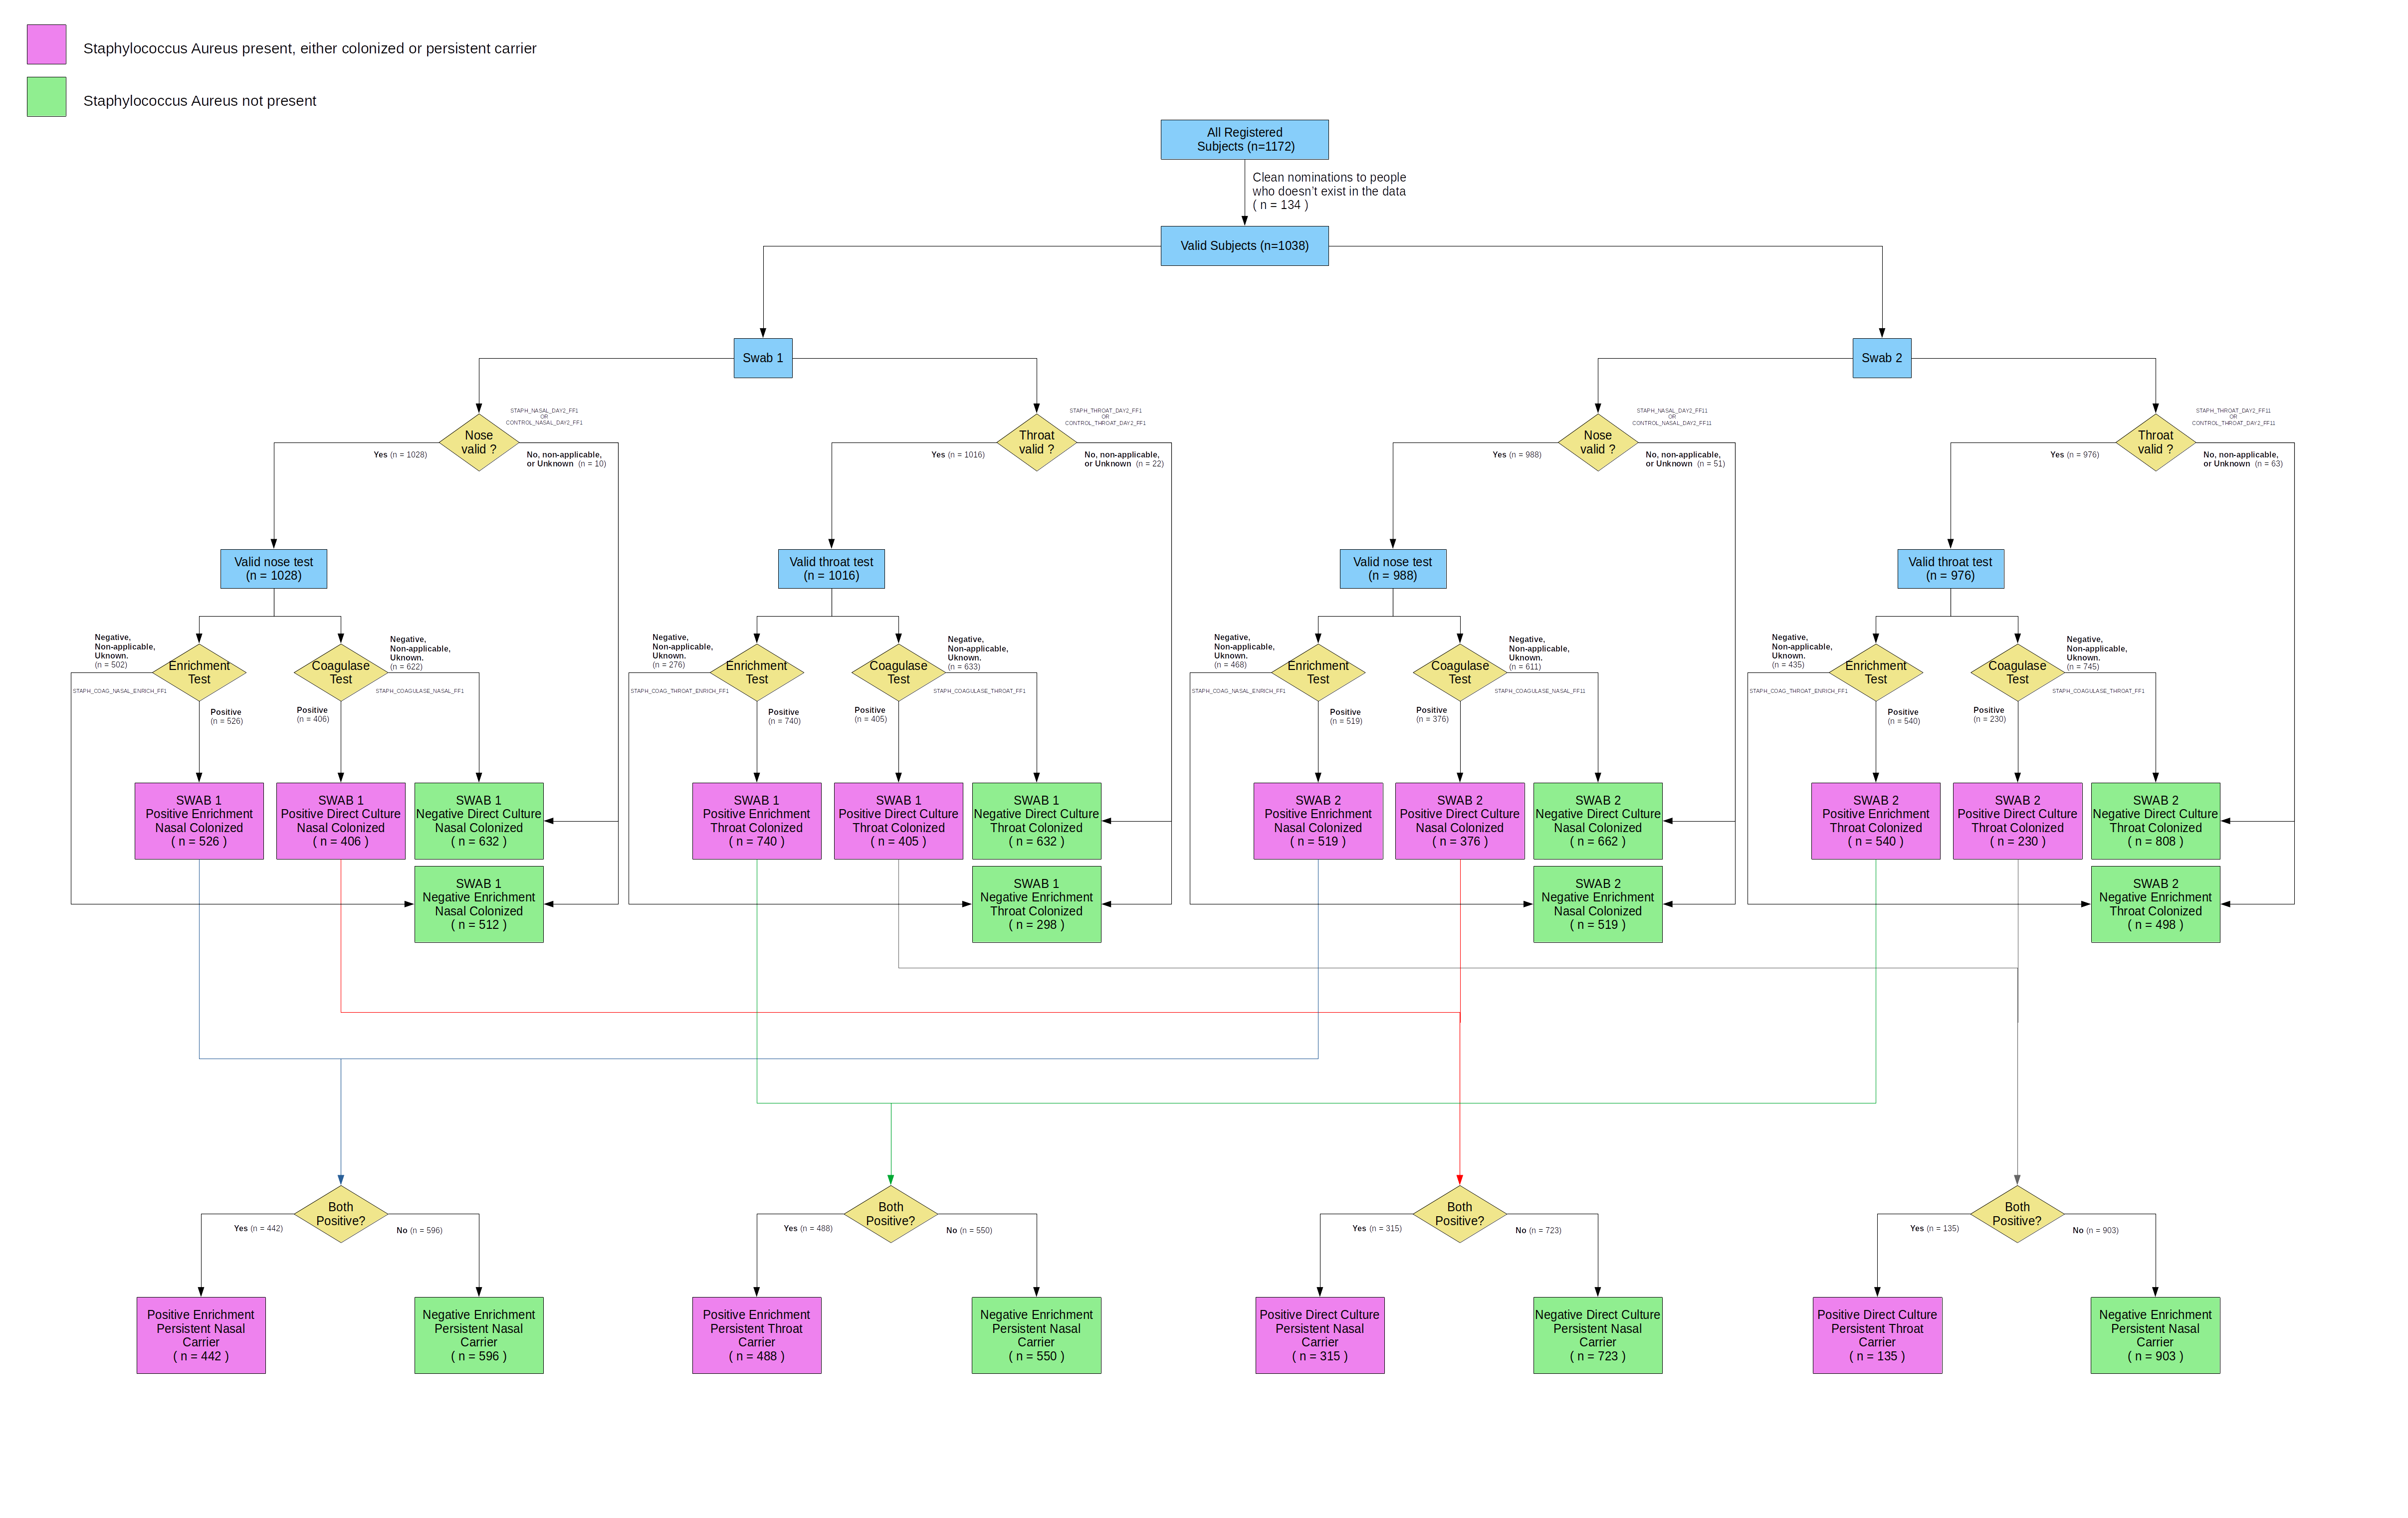
\includegraphics[width=1\textwidth]{../img/figures/carrierDefinition.png}
    \caption{Summarize of the definition of what is a nasal carrier subject. The throat definition follow the same scheme.}
}
\medskip
\end{figure}

	\textit{If we tried a test on the subject which show growing (“NasalGrowth” == “Yes”) and the coagulase test was ALSO positive (“CoagulaseNasal” == “Positive”), then we have a carrier.} \vspace{3 mm}

	The following figures illustrates which are considered carriers in the nose and the throat.\vspace{3 mm}

\input{../img/results/all/CategoricalHeatmap_aureusTable_NasalGrowth_CoagulaseNasal.tex}

\input{../img/results/all/CategoricalHeatmap_aureusTable_ThroatGrowth_CoagulaseThroat.tex}

	There are some minor inconsistencies in the data with this definition, which can be found in the following figures. But in the vast majority of the cases, all the control variables check-out correctly.\vspace{3 mm}

\input{../img/results/all/CategoricalHeatmap_aureusTable_NasalPopulation_CoagulaseNasal.tex}

\input{../img/results/all/CategoricalHeatmap_aureusTable_NasalPopulation_CoagulaseNasal.tex}
	
	We finally added another column to simplify everything, which tells you if you are S. Aureus carrier or not. This is positive if the nose is positive, or the throat is positive, and the other variable is not unknown. This is negative if both of them are negative. If either of them is unknown, this variable is unknown; but at the time of writing this, we have no such cases.\vspace{3 mm}



